% Made up for the tikra benchmark.
\usetikzlibrary{calc}
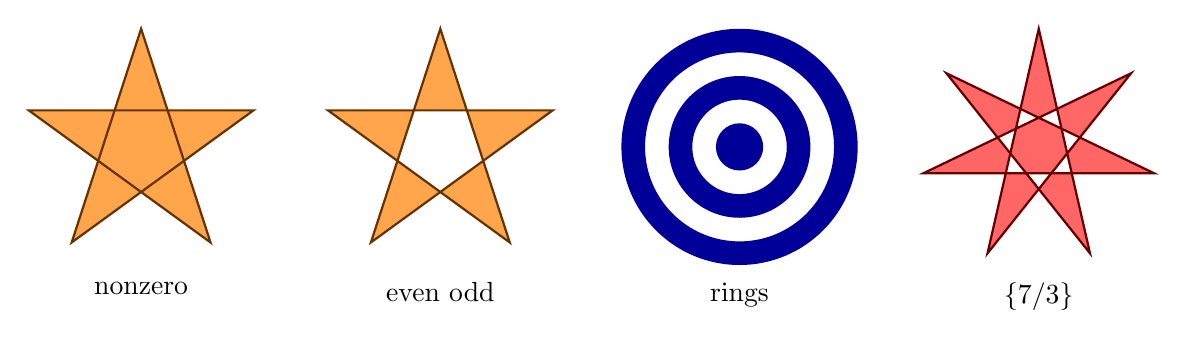
\begin{tikzpicture}
  % a pentagram: the nonzero rule fills the middle, the even odd rule leaves it empty
  \filldraw[fill=orange!70, draw=orange!40!black, thick]
    (90:1.5) -- (234:1.5) -- (18:1.5) -- (162:1.5) -- (306:1.5) -- cycle;
  \node[below] at (0,-1.6) {nonzero};
  \filldraw[fill=orange!70, draw=orange!40!black, thick, even odd rule, xshift=3.8cm]
    (90:1.5) -- (234:1.5) -- (18:1.5) -- (162:1.5) -- (306:1.5) -- cycle;
  \node[below] at (3.8,-1.6) {even odd};
  % concentric rings from one path
  \fill[blue!60!black, even odd rule] (7.6,0) circle (1.5) circle (1.2) circle (0.9) circle (0.6) circle (0.3);
  \node[below] at (7.6,-1.6) {rings};
  % a seven-pointed star polygon {7/3}
  \filldraw[fill=red!60, draw=red!40!black, thick, even odd rule]
    (11.4,0) ++(90:1.5) \foreach \k in {1,...,6} { -- ($(11.4,0)+(90+\k*154.2857:1.5)$) } -- cycle;
  \node[below] at (11.4,-1.6) {$\{7/3\}$};
\end{tikzpicture}
